% Début de la page de garde
\begin{titlepage}
  % Géométrie page de garde
  \newgeometry{
    top=20mm,
    bottom=25mm,
    left=15mm,
    right=15mm,
    nofoot,
    nohead,
    nomarginpar}
  \centering

  %%%%%%%%%%%%%%%%%%%%%%%%%%%%%%%%%%%%%%%%%%%%%%%%%%%%%%%%%%%%%%%%%% 
  %% Fond
  %%%%%%%%%%%%%%%%%%%%%%%%%%%%%%%%%%%%%%%%%%%%%%%%%%%%%%%%%%%%%%%%%% 
  % \begin{tikzpicture}[overlay,remember picture]
  \coordinate (SW) at (current page.south west);
  \coordinate (SE) at (current page.south east);
  \coordinate (NW) at (current page.north west);
  \coordinate (NE) at (current page.north east);

  % Affichage des noeuds
  \node[draw] at (SW) {};
  \node[draw] at (SE) {};
  \node[draw] at (NW) {};
  \node[draw] at (NE) {};


  \path (NE) -- (NW) node [pos=.3](P1){};
  \path (NW) -- (SW) node [pos=.3](P2){};
  \path (SE) -- (SW) node [pos=.3](P3){};
  \path (NE) -- (SE) node [pos=.3](P4){};


  \path[draw] (P2)--(P4) node[pos=.3](P5){};

  \path[draw, fill=blue] (P1) -- (P5);

  %\path[fill=blue] (SW) -- (NE) -- (SE) -- cycle;
  %\path[fill=red] (SW) -- (NE) -- (NW) -- cycle;
\end{tikzpicture}
  %%%%%%%%%%%%%%%%%%%%%%%%%%%%%%%%%%%%%%%%%%%%%%%%%%%%%%%%%%%%%%%%%% 
  %% Logos
  %%%%%%%%%%%%%%%%%%%%%%%%%%%%%%%%%%%%%%%%%%%%%%%%%%%%%%%%%%%%%%%%%% 
  % Les Fbox ne servent qu'au debug
  % \fbox{
  \begin{minipage}[t][3.5cm][t]{.95\textwidth}
    \hspace{.1cm}
    % \fbox{
    \begin{minipage}[c]{4cm}
      \centering
      
\includegraphics[width=4cm]{./figures/Logo_Univ.pdf}
    \end{minipage}
    \hfill
    \begin{minipage}[c]{4cm}
      \centering
      % Logo CHOUCAS
      
\includegraphics[width=4cm]{./figures/Logo_mstic.pdf}
    \end{minipage}
    \hfill
    % % \fbox{
    \begin{minipage}[c]{2cm}
      \centering
      % Logo CHOUCAS
      
\includegraphics[width=2cm]{./figures/logo-choucas.png}
    \end{minipage}
    \hfill
    % % }
    %   \fbox{
    \begin{minipage}[c]{2cm}
      \centering
      % Logo IGN
      \includegraphics[width=2cm]{./figures/Logo_ign.pdf}
      % Logo Lastig
      % 
\includegraphics[width=2cm]{./figures/logo-choucas.png}
    \end{minipage}
    % }
    \hspace{.1cm}
  \end{minipage}
  % }
  \par
  %%%%%%%%%%%%%%%%%%%%%%%%%%%%%%%%%%%%%%%%%%%%%%%%%%%%%%%%%%%%%%%%%% 
  %% Descriptif
  %%%%%%%%%%%%%%%%%%%%%%%%%%%%%%%%%%%%%%%%%%%%%%%%%%%%%%%%%%%%%%%%%% 
  \vspace{.05\textheight}
  % \fbox{
  \begin{minipage}{0.7\textwidth}
    \centering
    % Pour l'obtention
    {\usekomafont{subtitle} Thèse de doctorat\par} \vspace{.01\textheight}
    {\usekomafont{titlehead} Spécialité : Sciences et technologies de
      l'information Géographique }
  \end{minipage}
  % }
  \par
  \vfill
  % \vspace{.025\textheight}
  {\usekomafont{author} Mattia Bunel}\par
  \vspace{.05\textheight}
  %%%%%%%%%%%%%%%%%%%%%%%%%%%%%%%%%%%%%%%%%%%%%%%%%%%%%%%%%%%%%%%%%% 
  %% Titre
  %%%%%%%%%%%%%%%%%%%%%%%%%%%%%%%%%%%%%%%%%%%%%%%%%%%%%%%%%%%%%%%%%% 
  % \fbox{
  \begin{minipage}{0.95\textwidth}
    \centering
    % Titre
    {\usekomafont{title}\Huge Modélisation et raisonnement spatial
      imprécis pour l'aide à la localisation de victimes en
      montagne \par}
  \end{minipage}
  % }
  \vfill
  %%%%%%%%%%%%%%%%%%%%%%%%%%%%%%%%%%%%%%%%%%%%%%%%%%%%%%%%%%%%%%%%%% 
  %% Illustration
  %%%%%%%%%%%%%%%%%%%%%%%%%%%%%%%%%%%%%%%%%%%%%%%%%%%%%%%%%%%%%%%%%% 
  \begin{tikzpicture}
  \begin{scope}[local bounding box=obr]
    \fill[ffa] (1.125,.375) circle [radius=3pt];
    \path[ffc] (1.125,.375) circle [radius=3pt];
    \path[ffc] (0,0) rectangle (2,2);
  \end{scope}
  \begin{scope}[xshift=4.25cm]
    \begin{scope}
      \foreach \x in {0,.25,...,1.75}{
        \foreach \y in {0,.25,...,1.75}
        \path[draw, line width=.01mm] (\x,\y) rectangle (\x +.25, \y + .25);
      }
      \path[ffa] (1,.25) rectangle (1.25, .5);
      \path[ffc] (0,0) rectangle (2,2);
    \end{scope}
  \end{scope}
  \begin{scope}[xshift=8.5cm,local bounding box=met]
    \begin{scope}
      \foreach \x in {0,.25,...,1.75}{
        \foreach \y in {0,.25,...,1.75}
        {
          \path[draw, line width=.01mm] (\x,\y) rectangle (\x +.25, \y +
          .25);
          \pgfmathsetmacro\radius{sqrt((\x-1.125)^2+(\y-.375)^2)*1.25}
          \fill[black] (\x+.125,.125+\y) circle (\radius pt);
        }
      }
      \path[ffc] (0,0) rectangle (2,2);
    \end{scope}
  \end{scope}
  \begin{scope}[xshift=12.75cm,local bounding box=fuzz]
    \begin{scope}
      \foreach \x in {0,.25,...,1.75}{
        \foreach \y in {0,.25,...,1.75}
        {
          \path[draw, line width=.01mm] (\x,\y) rectangle (\x +.25, \y +
          .25);
          \pgfmathsetmacro\dist{sqrt((\x-1.125)^2+(\y-.375)^2)}
          \pgfmathsetmacro\fuzzy{%
            ifthenelse(\dist < .25,1,%
            ifthenelse(\dist < 2,-0.57*\dist+1.14,0)%
            )
          }
          \pgfmathsetmacro\radius{\fuzzy*2.5}
          \fill[black] (\x+.125,.125+\y) circle (\radius pt);
        }
      }
      \path[ffc] (0,0) rectangle (2,2);
    \end{scope}
  \end{scope}
  \begin{scope}
    \path[draw, ->] (2.5,1) --++ (1.25,0);
    \path[draw, ->] (6.75,1) --++ (1.25,0);
    \path[draw, ->] (11,1) --++ (1.25,0);
  \end{scope}
\end{tikzpicture}
  % 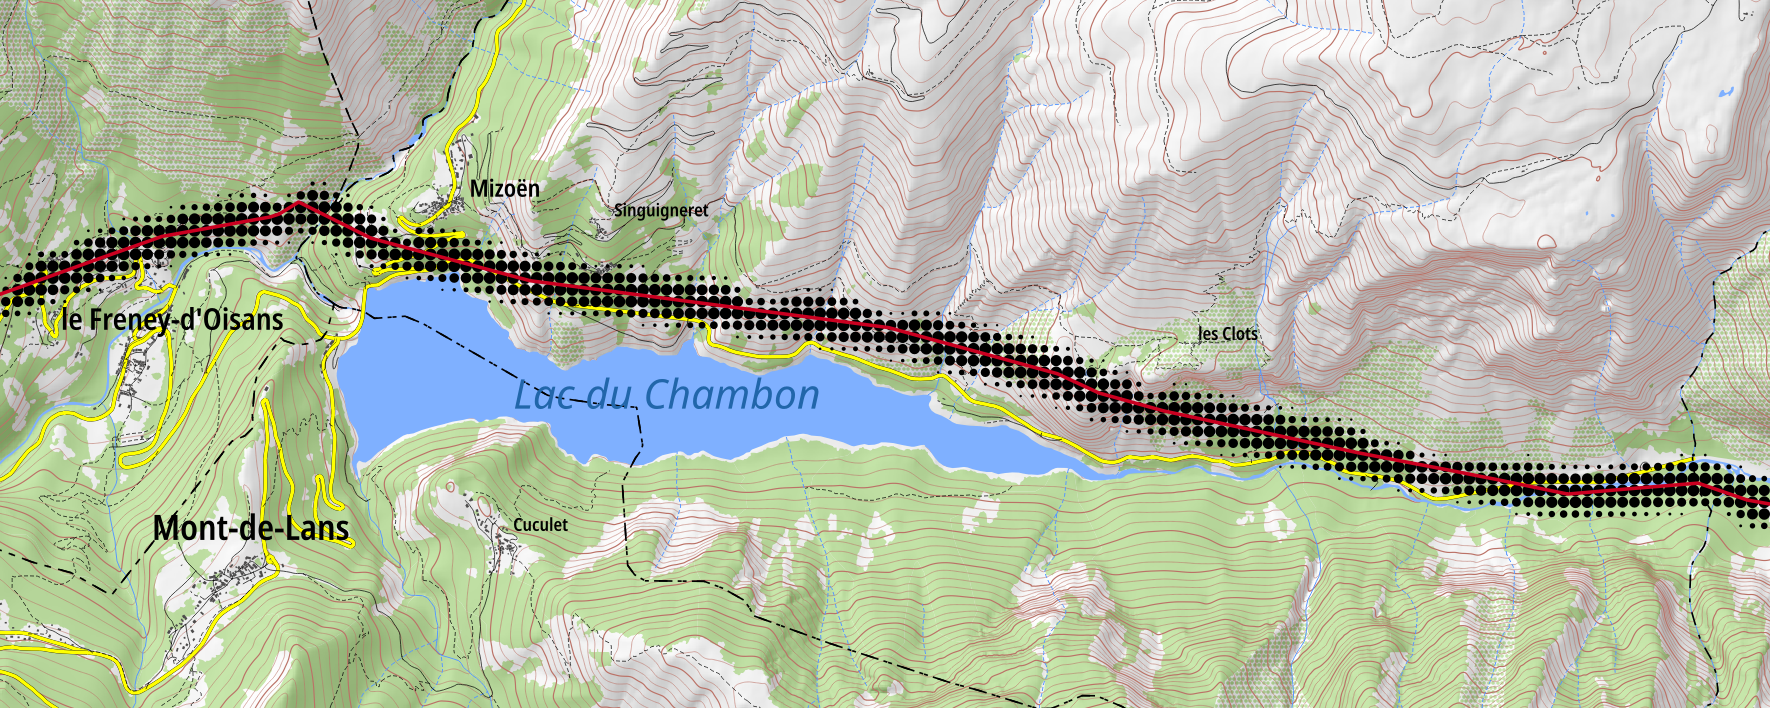
\includegraphics{./figures/Raster_ZLP_SOUS_HT.png}
  \vfill
  \noindent
  %%%%%%%%%%%%%%%%%%%%%%%%%%%%%%%%%%%%%%%%%%%%%%%%%%%%%%%%%%%%%%%%%% 
  %% Jury
  %%%%%%%%%%%%%%%%%%%%%%%%%%%%%%%%%%%%%%%%%%%%%%%%%%%%%%%%%%%%%%%%%% 
  % \fbox{
  \begin{minipage}[t]{0.95\textwidth}
    \centering Soutenue publiquement le 19 février 2021 devant un jury
    composé de :\par
    \vspace{.01\textheight} {\footnotesize
      \begin{tabular}{m{0.95\textwidth}}
        M\up{me} Mireille \bsc{Batton-Hubert}, Professeure, École des Mines de Saint-Étienne \dotfill Rapportrice\\
        % 
        M\up{me} Sophie \bsc{de Ruffray}, Professeure, Université de Rouen--Normandie \dotfill Rapportrice\\
        % 
        M. Thomas \bsc{Devogele}, Professeur, Université François Rabelais de Tours  \dotfill Examinateur\\
        % 
        M\up{me} Cécile \bsc{Duchêne}, Enseignante-Chercheuse (HDR),
        IGN (Saint-Mandé) \dotfill Directrice de thèse\\
        % 
        M. Olivier \bsc{Favre}, PGHM de Grenoble \dotfill Invité\\
        % 
        M. Didier \bsc{Josselin}, Directeur de recherche, CNRS--UMR Espace (Avignon) \dotfill Examinateur\\
        % 
        M\up{me} Ana-Maria \bsc{Olteanu-Raimond}, Chargée de recherche (HDR), IGN (Saint-Mandé)\dotfill Directrice de thèse\\
      \end{tabular}
    }
  \end{minipage}
  \vfill
  \centering
  {\usekomafont{titlehead} Université Gustave Eiffel --- École doctorale MSTIC}\par
  {\usekomafont{titlehead} Institut national de l'information
    géographique et forestière --- UMR LASTIG}\par
\end{titlepage}

% Retour à la géométrie initiale
\restoregeometry